% Author: Alejandro Santomé Valverde


\chapter{Optimization and Characterization of Fundamental SOI Building Blocks}\label{chap:blocks} % (fold)

\section{Introduction to the Fabrication Platform} \label{sec:fabrication_platform}

The realization of the programmable photonic circuits discussed in this thesis relies on the 
maturity and precision of the Silicon-on-Insulator platform. This section details the technological 
framework, the computational tools employed for device optimization, and the experimental 
infrastructure used to validate the performance of the fundamental building blocks.

\subsection{SOI Fabrication Platforms} \label{subsec:foundry}

The devices characterized in this work were fabricated using \textbf{dedicated wafer runs} across 
different fabrication facilities. The use of dedicated runs allowed for full-wafer layout control 
and the implementation of specific process optimizations tailored to the requirements of 
large-scale programmable architectures. 

The baseline platform consists of a standard SOI wafer with a nominal silicon device layer 
thickness of $220$~nm, resting on a thick Buried Oxide (BOX) layer that ensures modal isolation 
from the handle substrate. To ensure portability across different manufacturing environments, the 
building blocks were adapted to the specific Process Design Kits (PDKs) and design rules of each 
foundry. This included adjustments in the slab thickness for rib geometries (typically ranging 
between $70$~nm and $90$~nm) and and the re-optimization of critical dimensions to comply with 
fabrication constraints, such as the minimum achievable tip width for the silicon waveguides.

Furthermore, the designs account for the specific Back-End-Of-Line (BEOL) stack of each process. 
The vertical distance and composition of the dielectric cladding and metal layers were critical 
parameters for the optimization of active components, such as thermo-optic phase shifters, ensuring 
that the building blocks remain compatible with the multi-layer metal routing required for 
large-scale system integration.

\subsection{Design and Simulation Workflow} \label{subsec:workflow}

The transition from theoretical concepts to physical layout follows a rigorous multi-step 
simulation and optimization workflow. The choice of numerical method was strategically dictated 
by the physical dimensions and the nature of the light-matter interaction in each building block 
to balance computational efficiency and accuracy.

\begin{itemize}
    \item \textbf{Waveguide and Modal Analysis:} The fundamental propagation properties, including 
    effective indices ($n_{eff}$) and group indices ($n_g$), were analyzed using Finite Difference 
    Eigenmode (FDE) solvers. This analysis provided the necessary baseline for phase shifter 
    designs and established the confinement conditions across the different SOI platforms used.
    
    \item \textbf{Edge Coupler Simulation (BPM):} Given the relatively large longitudinal 
    dimensions of the spot-size converters---typically in the order of hundreds of 
    micrometers---the Beam Propagation Method (BPM) was employed. Specifically, Synopsys RSoft 
    BeamPROP was used to simulate the adiabatic expansion of the mode along the inverted tapers. 
    This approach allowed for an efficient evaluation of coupling efficiency and modal evolution, 
    providing a reliable design framework with a significantly lower computational cost than 
    full-wave methods.
    
    \item \textbf{MMI Optimization (FDTD):} For the design of compact and high-performance MMI 
    couplers, where scattering and multi-mode interference effects are dominant, the 
    Finite-Difference Time-Domain (FDTD) method was utilized via Ansys Lumerical. This solver 
    provides the necessary precision to capture broadband responses and complex phase 
    relationships. Furthermore, the Adjoint optimization method was integrated into the FDTD 
    workflow to explore a high-dimensional design space, resulting in the optimized geometries 
    discussed in Section \ref{sec:mmi_adjoint}.
    
    \item \textbf{Layout Generation:} Once the design targets were achieved, the device geometries 
    were translated into GDSII files. Depending on the specific fabrication run and circuit 
    complexity, layouts were generated using Synopsys OptoDesigner for certain designs, while the 
    Python-based framework gdsfactory was utilized for others. These tools enabled script-based 
    generation to ensure sub-nanometer precision in the definition of adiabatic curves and complex 
    optimized shapes, with KLayout serving as the primary environment for final inspection and 
    design rule verification.
\end{itemize}

Other specialized components, such as Arrayed Waveguide Gratings (AWGs), required dedicated 
simulation approaches tailored to their specific dispersive properties. For these devices, the 
EPIPProp tool from Photon Design was employed, which provides a specialized framework for modeling 
the complex phase and amplitude relationships in waveguide-array-based structures. Further details 
on these designs will be provided in their respective sections later in this work.



\subsection{Experimental Characterization Setup} \label{subsec:setup}

To validate the performance of the designed building blocks, two distinct experimental 
characterization benches were employed. Both setups share a common optical backbone consisting of a 
tunable CW laser source, a polarization controller to excite the fundamental TE mode, and 
high-sensitivity power meters. The choice between these setups depends on whether the 
characterization requires high flexibility for active tuning or statistical data through 
high-throughput measurements.

\subsubsection{Single Input-Single Output (SISO) Setup}

\begin{figure}[!h]
    \centering
    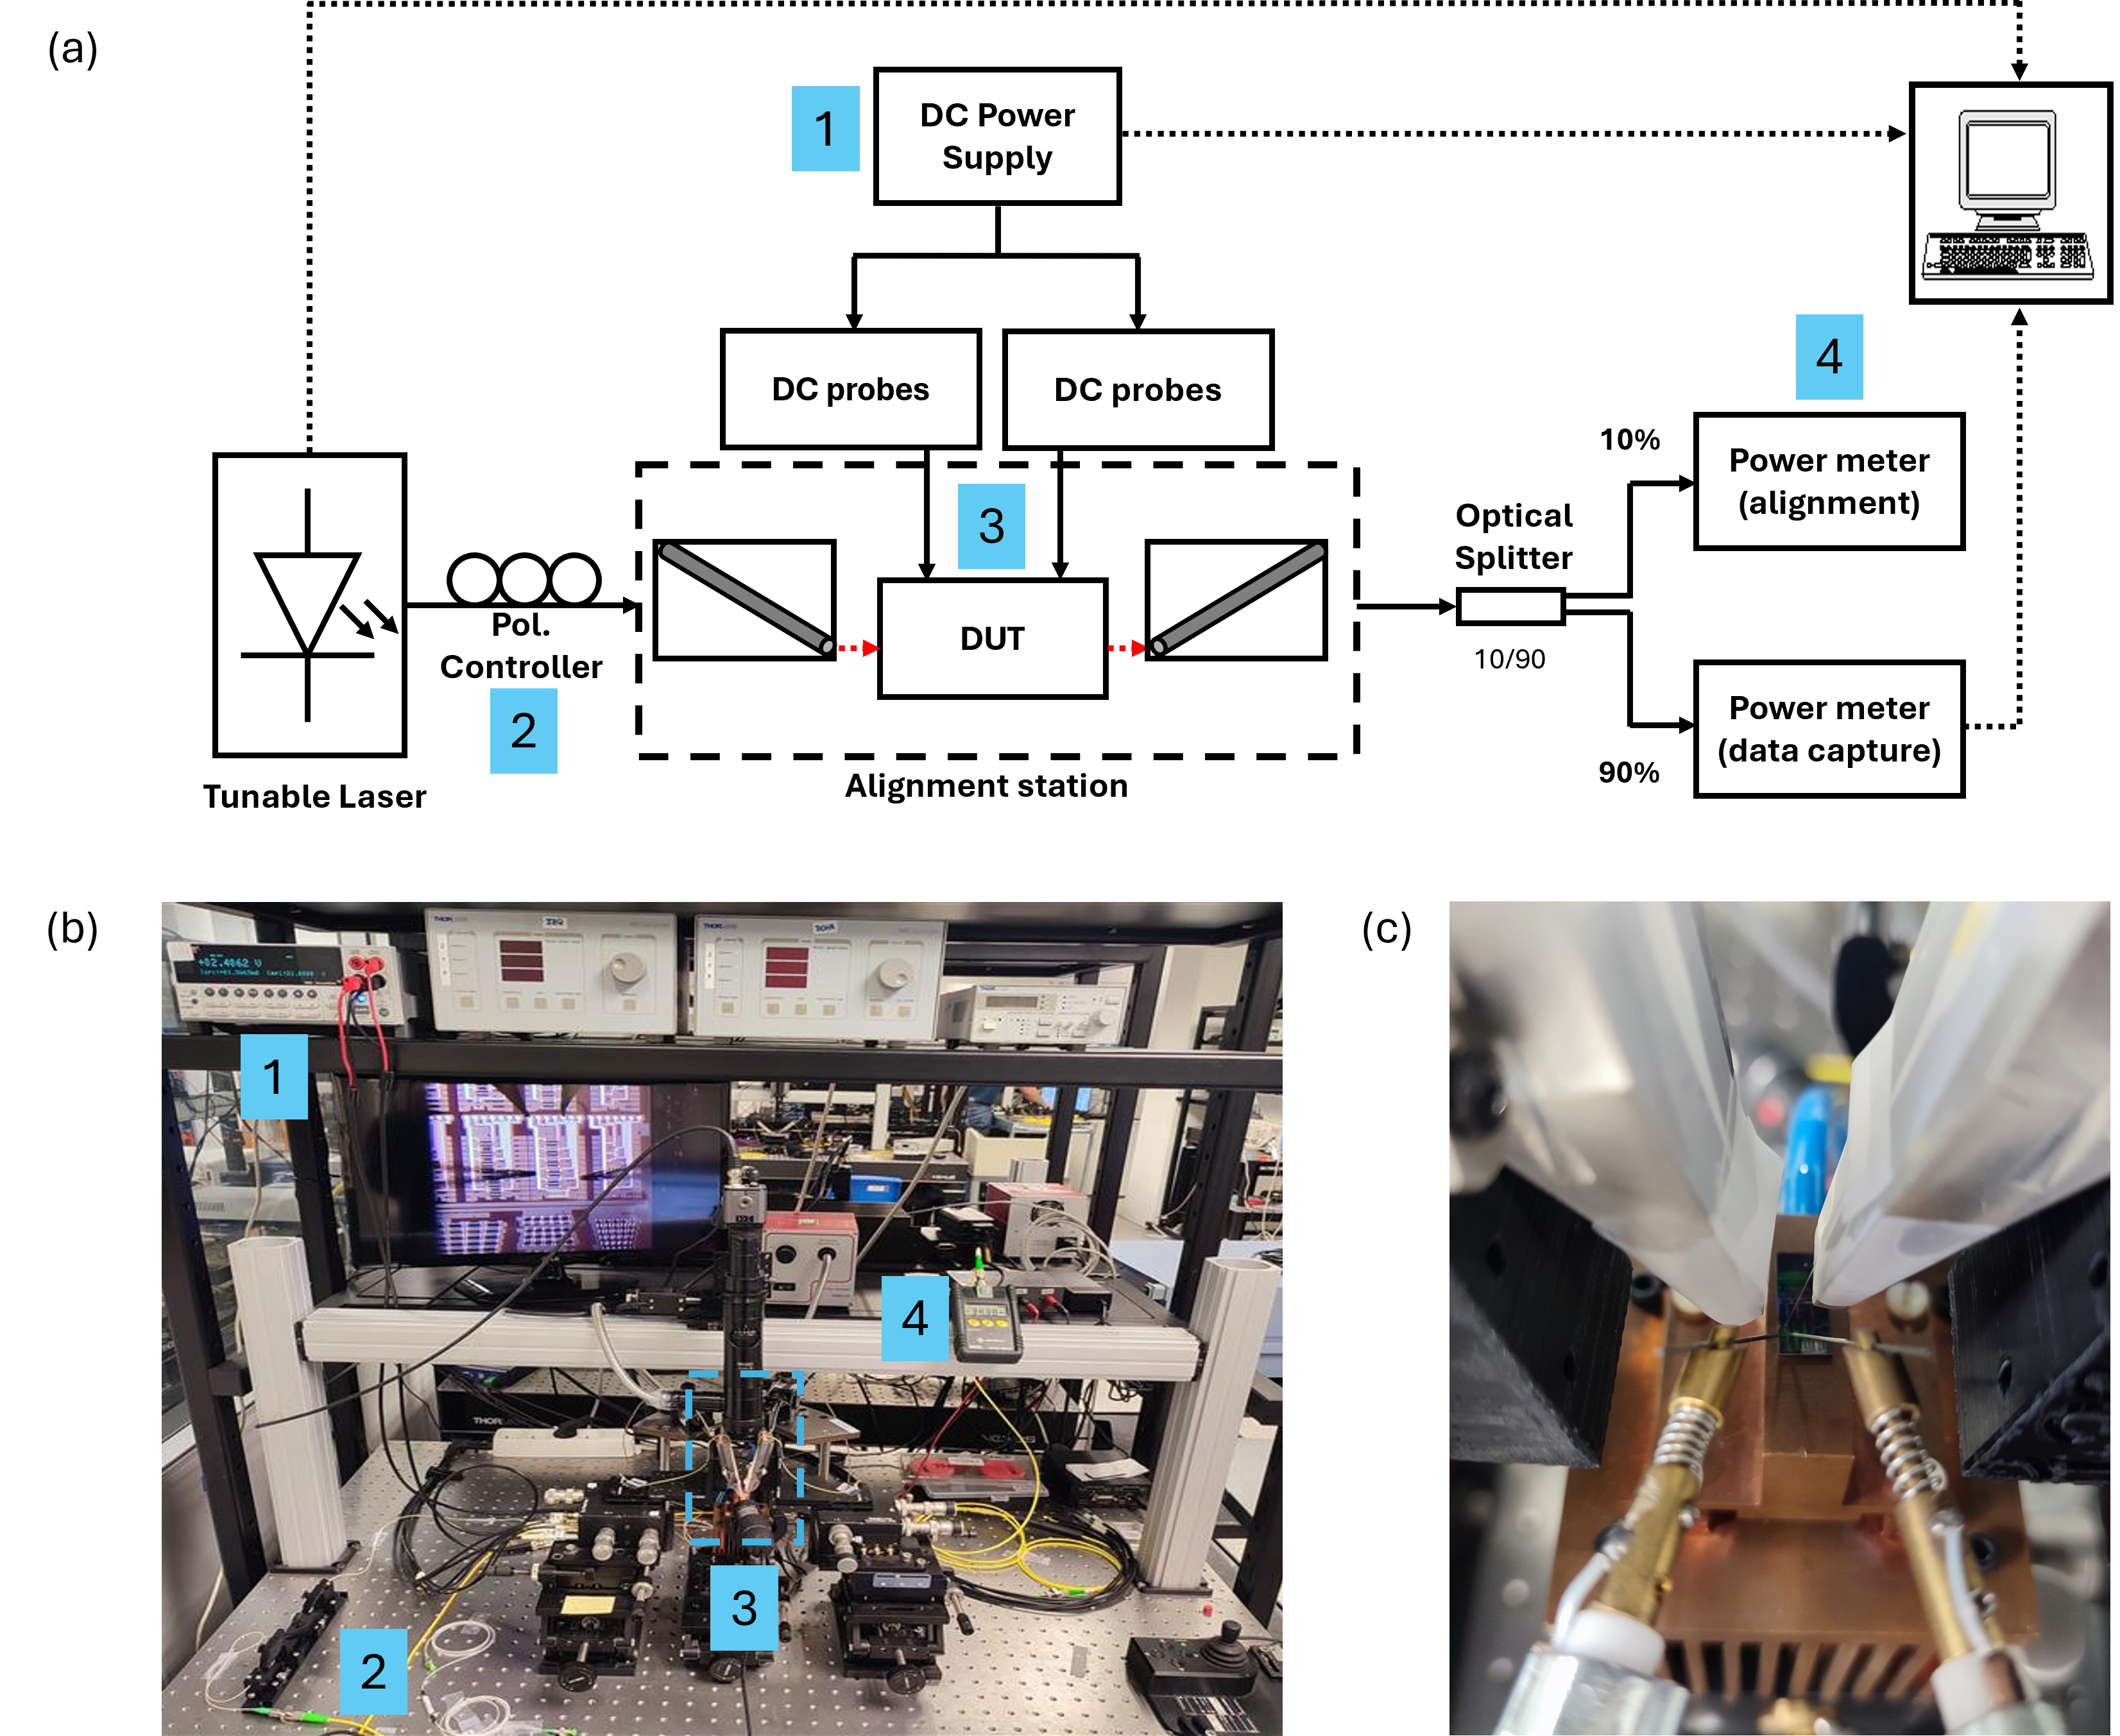
\includegraphics[width=\textwidth]{figures/ch3-siso_setup.png}
    \caption{SISO characterization bench: (a) Schematic representation showing the stages for edge 
    and vertical fiber coupling. (b) Photograph of the experimental setup, where the dashed cyan 
    box highlights the region detailed in the inset. (c) Close-up of the chip showing vertical 
    fiber alignment and DC probe needles for electrical excitation}
    \label{fig:ch3-siso_setup}
\end{figure}

The first setup is designed for maximum flexibility, allowing for the characterization of 
individual components and test structures. As illustrated in the schematic of Figure 
\ref{fig:ch3-siso_setup}a, the bench features high-precision motorized stages for coarse 
positioning, which are complemented by piezoelectric actuators for fine alignment. This 
sub-micrometric control is essential for maximizing coupling efficiency, particularly when dealing 
with the narrow mode-field diameters of edge couplers.

The setup can be configured for two primary coupling geometries:
\begin{itemize}
    \item \textbf{Edge Coupling:} Horizontal alignment using cleaved SMF-28 fibers to interface 
    with the spot-size converters at the chip facet.
    \item \textbf{Vertical Coupling:} Out-of-plane alignment for devices featuring grating 
    couplers.
\end{itemize}

The physical implementation is shown in Figure \ref{fig:ch3-siso_setup}b. This setup serves as the 
primary station for the characterization of active components. A dashed cyan box highlights the 
interaction area between the optical and electrical probes, which is further detailed in the inset 
of Figure \ref{fig:ch3-siso_setup}c. This close-up view shows the vertical fiber alignment and the 
two DC probe needles used to provide the electrical excitation to the thermo-optic phase shifters, 
a configuration required to characterize tuning efficiency and phase-power relationships.



\subsubsection{High-Throughput Semi-Automated Setup}

\begin{figure}[!ht]
    \centering
    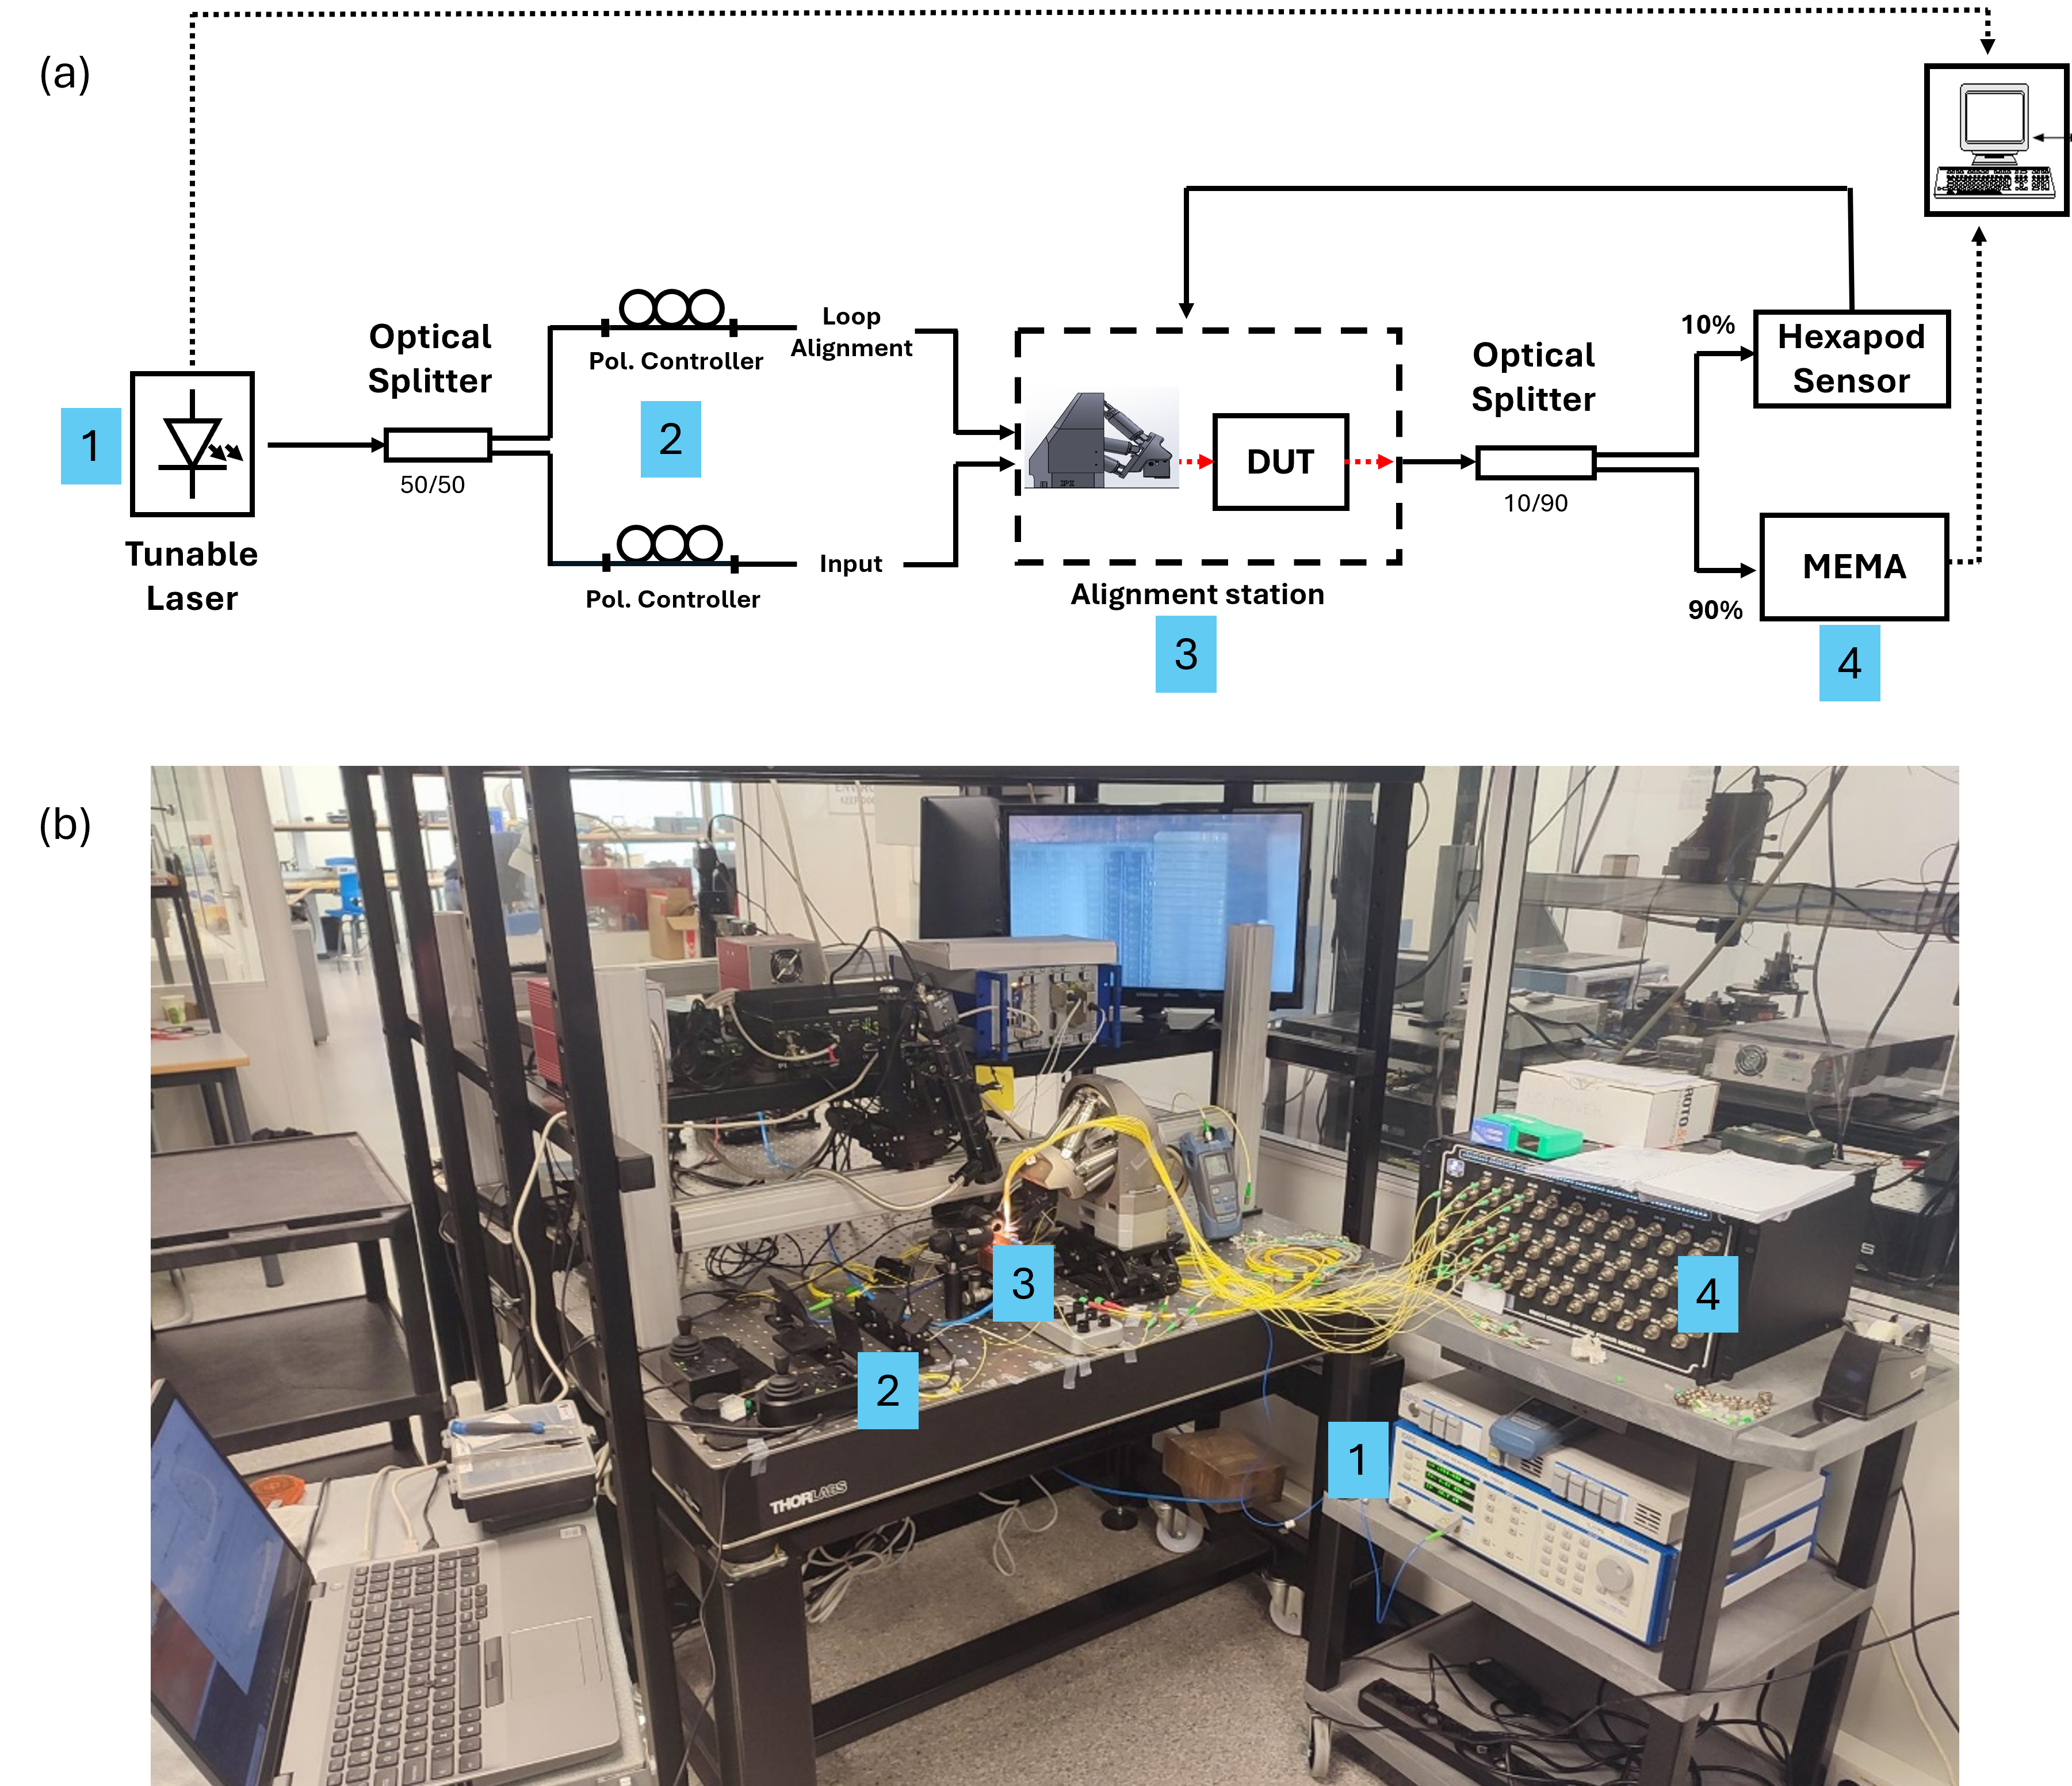
\includegraphics[width=\textwidth]{figures/ch3-hexapod_setup.png}
    \caption{High-throughput semi-automated characterization bench: (a) Schematic representation 
    showing the 64-channel fiber array and the hexapod positioner. (b) Photograph of the 
    experimental setup during the measurement of cascaded MMI 2x2 splitters.}
    \label{fig:ch3-hexapod_setup}
\end{figure}

For the precise extraction of performance metrics in passive components, such as the excess loss 
and imbalance of MMI couplers, a high-throughput setup is utilized. As shown in the schematic of 
Figure \ref{fig:ch3-hexapod_setup}a, this bench is equipped with a 64-channel fiber array mounted 
on a high-precision hexapod positioner, enabling semi-automated alignment routines.

The physical implementation is captured in Figure \ref{fig:ch3-hexapod_setup}b during the 
characterization of cascaded structures. By measuring chains of 16 to 18 cascaded MMIs, the 
cumulative loss can be determined with significantly reduced experimental error. This statistical 
approach allows for the extraction of the mean insertion loss per component through linear 
regression of the cascaded stages, effectively filtering out fluctuations from single-device 
measurements and fiber-to-chip coupling variations.

\subsubsection{Thermal Management and Stability}

Given the high thermo-optic coefficient of silicon \cite{cocorullo2002measurement}, all 
measurements were conducted under strict thermal control to prevent unwanted spectral shifts and 
ensure the reliability of the experimental data. The photonic chips were mounted on a specialized 
vacuum chuck equipped with a high-power Thermo-Electric Cooler (TEC) and a feedback thermistor. 
This closed-loop system ensures a constant operating temperature, typically maintained at 
$25^{\circ}\text{C}$ or $45^{\circ}\text{C}$. This stabilization is critical to avoid the drift of 
resonant structures and to ensure the repeatability of the results across different fabrication 
runs and measurement sessions.


\section{Simple Inverted Taper for Edge Coupling} \label{sec:taper}

While grating couplers offer high flexibility for wafer-level testing, they present significant 
limitations for certain advanced packaging paradigms. Specifically, the vertical emission of 
grating couplers is often incompatible with flip-chip bonding architectures, where the top 
surface of the photonic chip is obstructed by a mounted electronic or laser die. To overcome this 
and enable the ultra-dense integration required for the systems described in \ref{chap:systems}, a 
side-coupling approach using a simple inverted taper was implemented.


\subsection{Design Rationale and Geometry}

The edge coupler design is dictated by the specific layer stack and the lithographic constraints of 
the SOI foundry used in this work. Figure \ref{fig:ch3-taper_design}(a) illustrates the particular
cross-section of the platform, while Figure \ref{fig:ch3-taper_design}(b) presents the top-view 
geometry of the implemented inverted taper.

\begin{figure}[!ht]
    \centering
    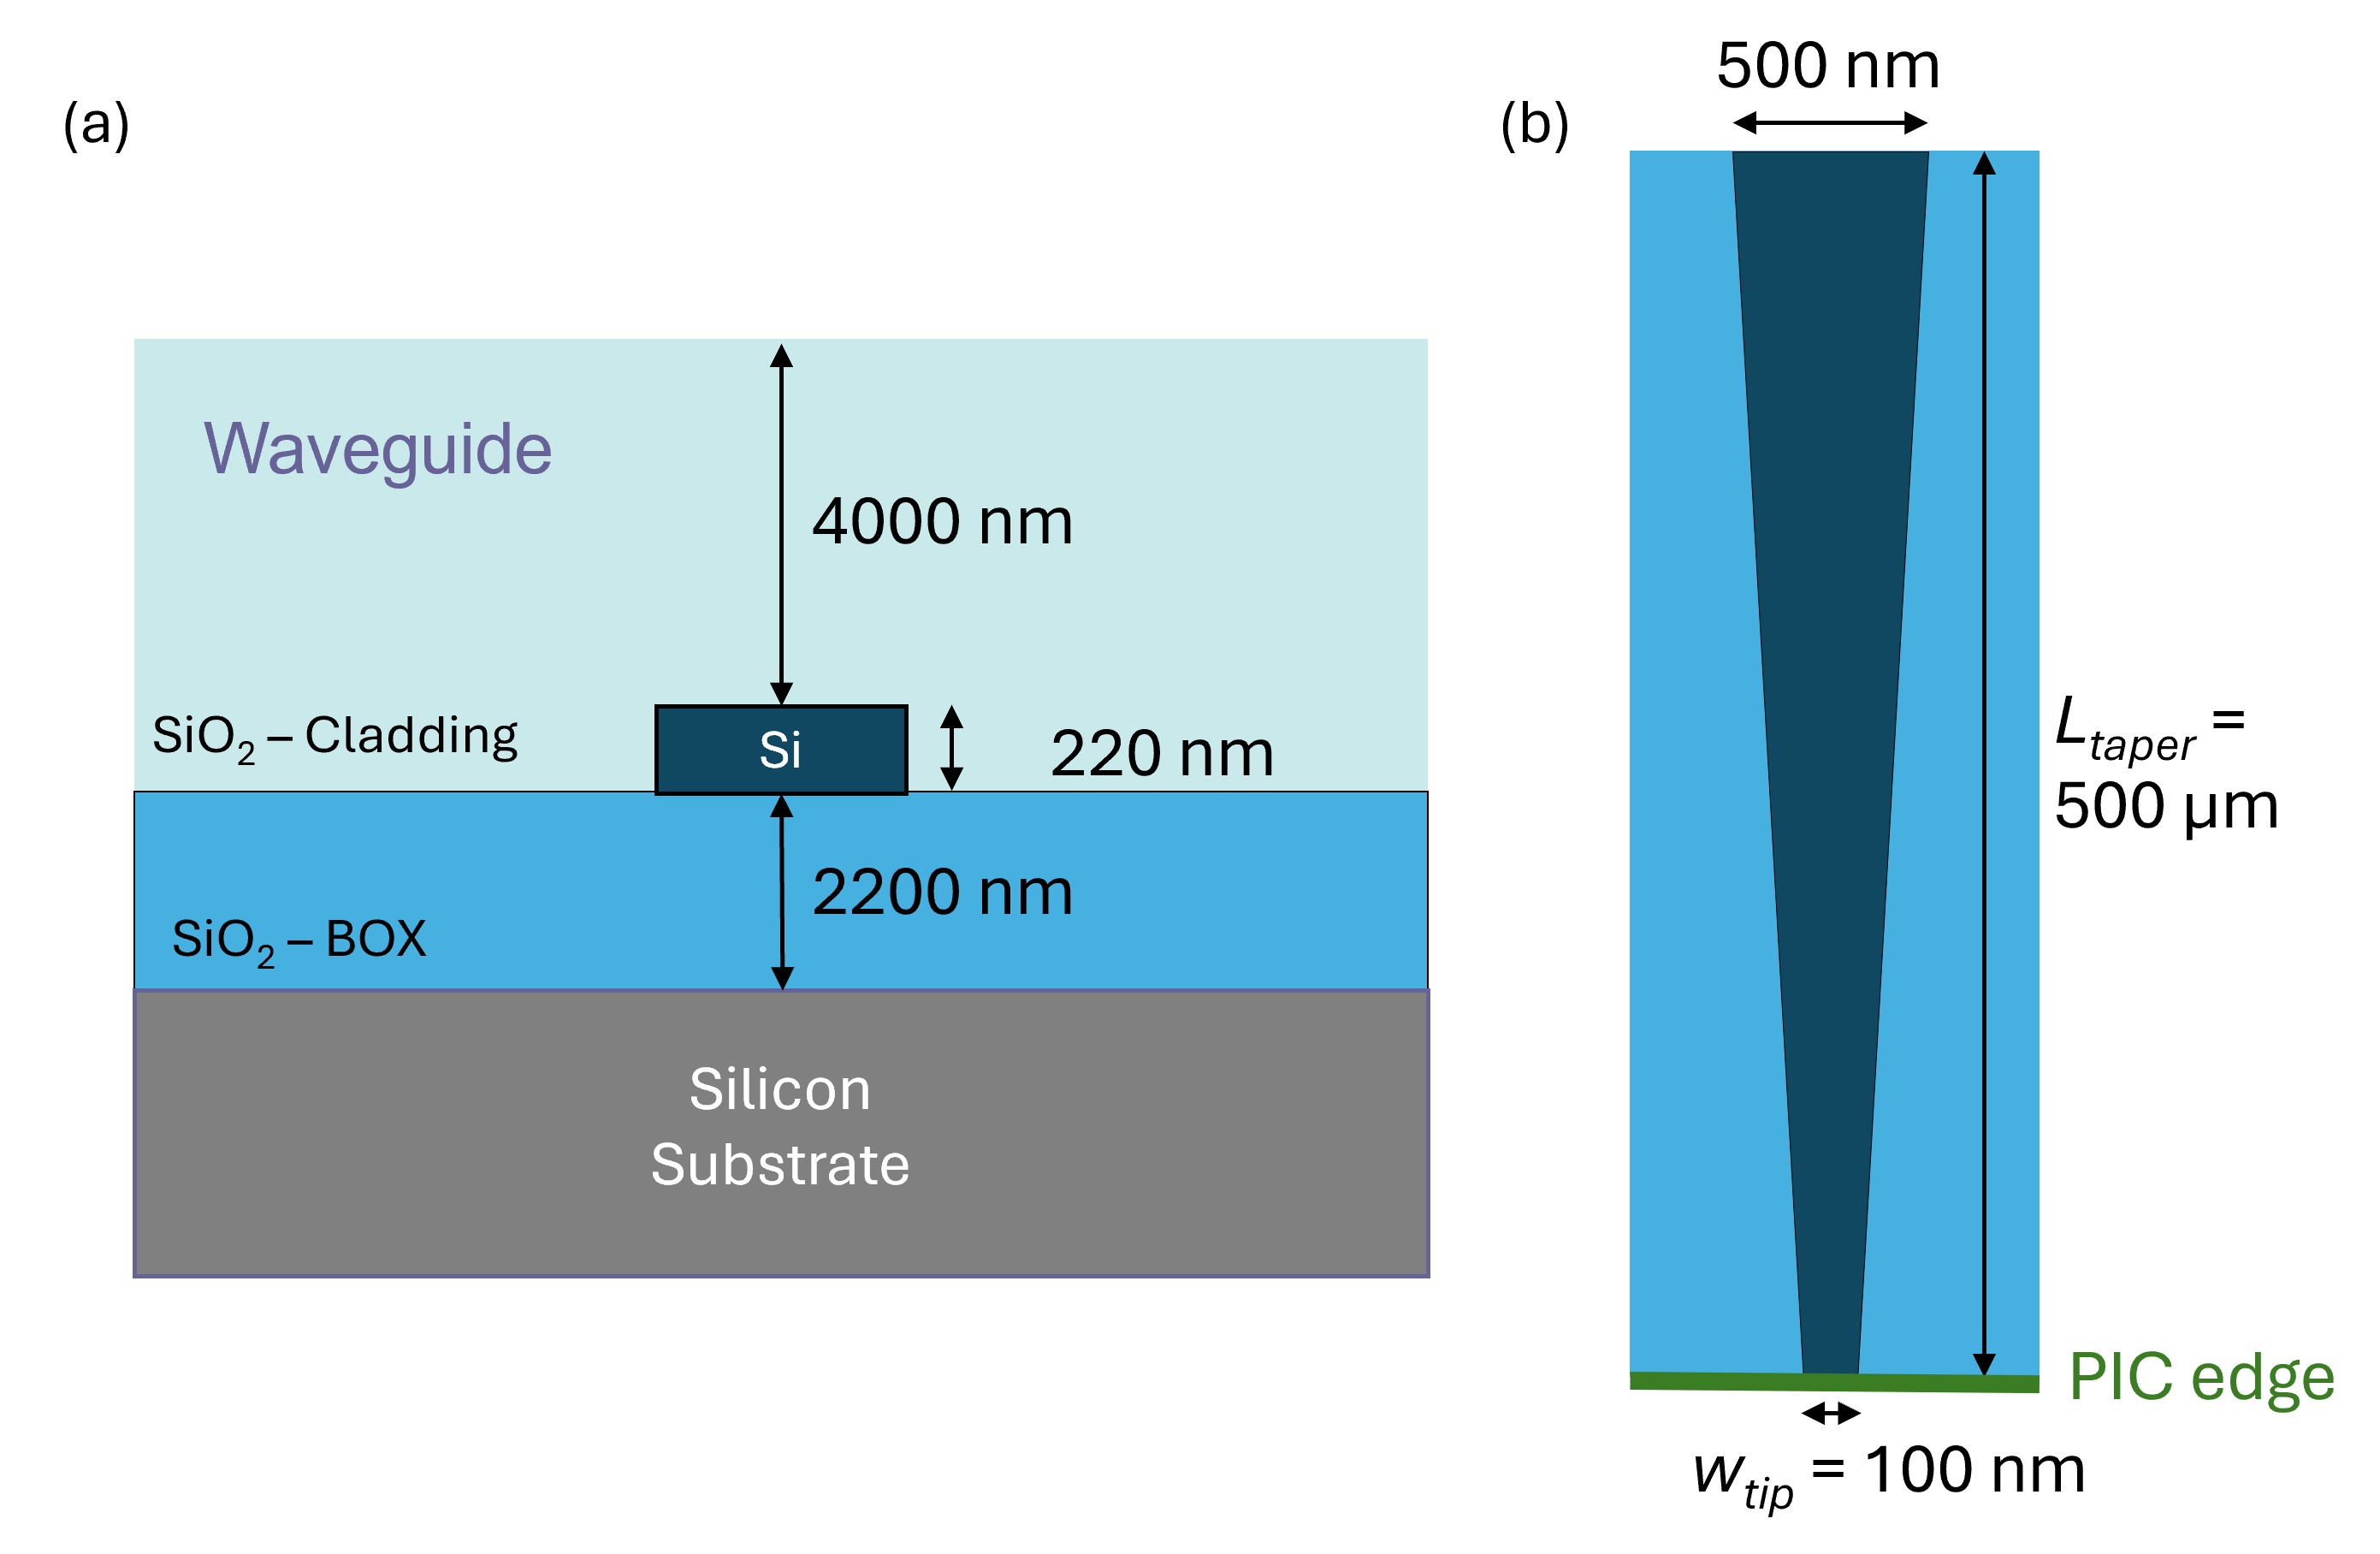
\includegraphics[width=0.7\textwidth]{figures/ch3-edge_coupler_design.png}
    \caption{Geometry of the inverted taper edge coupler: (a) Cross-section of the SOI stack 
    provided by the foundry. (b) Top-view of the $500 \ \mu\text{m}$ long linear taper 
    transitioning from the bus waveguide to the $100 \text{ nm}$ tip. Note: Dimensions in (b) are 
    not to scale.}
    \label{fig:ch3-taper_design}
\end{figure}

The physical dimensions of the SSC were selected to maximize mode expansion at the chip facet 
within the following foundry-specific parameters:
\begin{itemize}
    \item \textbf{Waveguide Stack:} The $220 \text{ nm}$ thick silicon core sits on a $2200 
    \text{ nm}$ BOX and is covered by a $4000 \text{ nm}$ $SiO_2$ upper cladding. This stack 
    thickness is critical as it defines the maximum volume available for the mode to expand as it 
    delocalizes from the silicon core.
    \item \textbf{Lithographic Limit ($w_{tip}$):} The width is reduced from the nominal 
    $500 \text{ nm}$ waveguide to a tip width of $100 \text{ nm}$. This is the minimum feature size
    allowed by the foundry's design rules, representing the narrowest possible tip to achieve the 
    highest MFD mismatch reduction.
    \item \textbf{Adiabatic Transition ($L_{taper}$):} A length of $500 \ \mu\text{m}$ was
    implemented to ensure an adiabatic modal transition. This length ensures that power is 
    transferred efficiently from the confined waveguide mode to the expanded cladding mode without 
    significant radiation losses.
\end{itemize}

As the device length is three orders of magnitude larger than its width, the schematic in Figure \ref{fig:ch3-taper_design}(b) uses a modified aspect ratio for clarity, focusing on the geometric transition rather than physical proportions.



\subsection{Simulation and Performance Baseline}

The design was simulated using the Beam Propagation Method (BPM) in RSoft to establish a 
performance baseline. Given that the focus of this work lies in the system-level integration rather 
than the optimization of the coupling interface itself, a straightforward linear geometry was 
prioritized for its fabrication robustness.
The simulation also pretends verifying the assumption that standard optical fibers are 
fundamentally mismatched with the mode expansion capabilities of a $100 \text{ nm}$ silicon tip. 
By establishing a performance baseline, we evaluate the necessity of employing specialized 
high-numerical aperture fibers and quantify the impact of fabrication tolerances.
Figure \ref{fig:ch3-taper_sims} summarizes the performance of the 
inverted taper regarding modal matching, spectral behavior, and dicing tolerances.

The relationship between fiber MFD and coupling efficiency, shown in Figure 
\ref{fig:ch3-taper_sims}(a), confirms that the delocalized mode at the $100 \text{ nm}$ tip is 
insufficient to match the $\sim 10.4 \ \mu\text{m}$ MFD of a standard SMF-28 fiber, resulting in 
losses above $4.25 \text{ dB}$. To validate the need for a specialized interface, we compared these 
results with Ultra-High Numerical Aperture (UHNA) fibers. As illustrated in the 
spectral response in Figure \ref{fig:ch3-taper_sims}(b), UHNA1 \cite{coherent_uhna1} 
($MFD \approx 4.8 \ \mu\text{m}$) provides the optimal match with an excess loss of approximately 
$2.5 \text{ dB}$ and a remarkably flat behavior across the C-band. In contrast, UHNA7 
\cite{coherent_uhna7} ($MFD \approx 3.2 \ \mu\text{m}$) shows higher losses due to 
over-confinement, confirming UHNA1 as the necessary bridge for this SOI interface.

\clearpage

\begin{figure}[!ht]
    \centering
    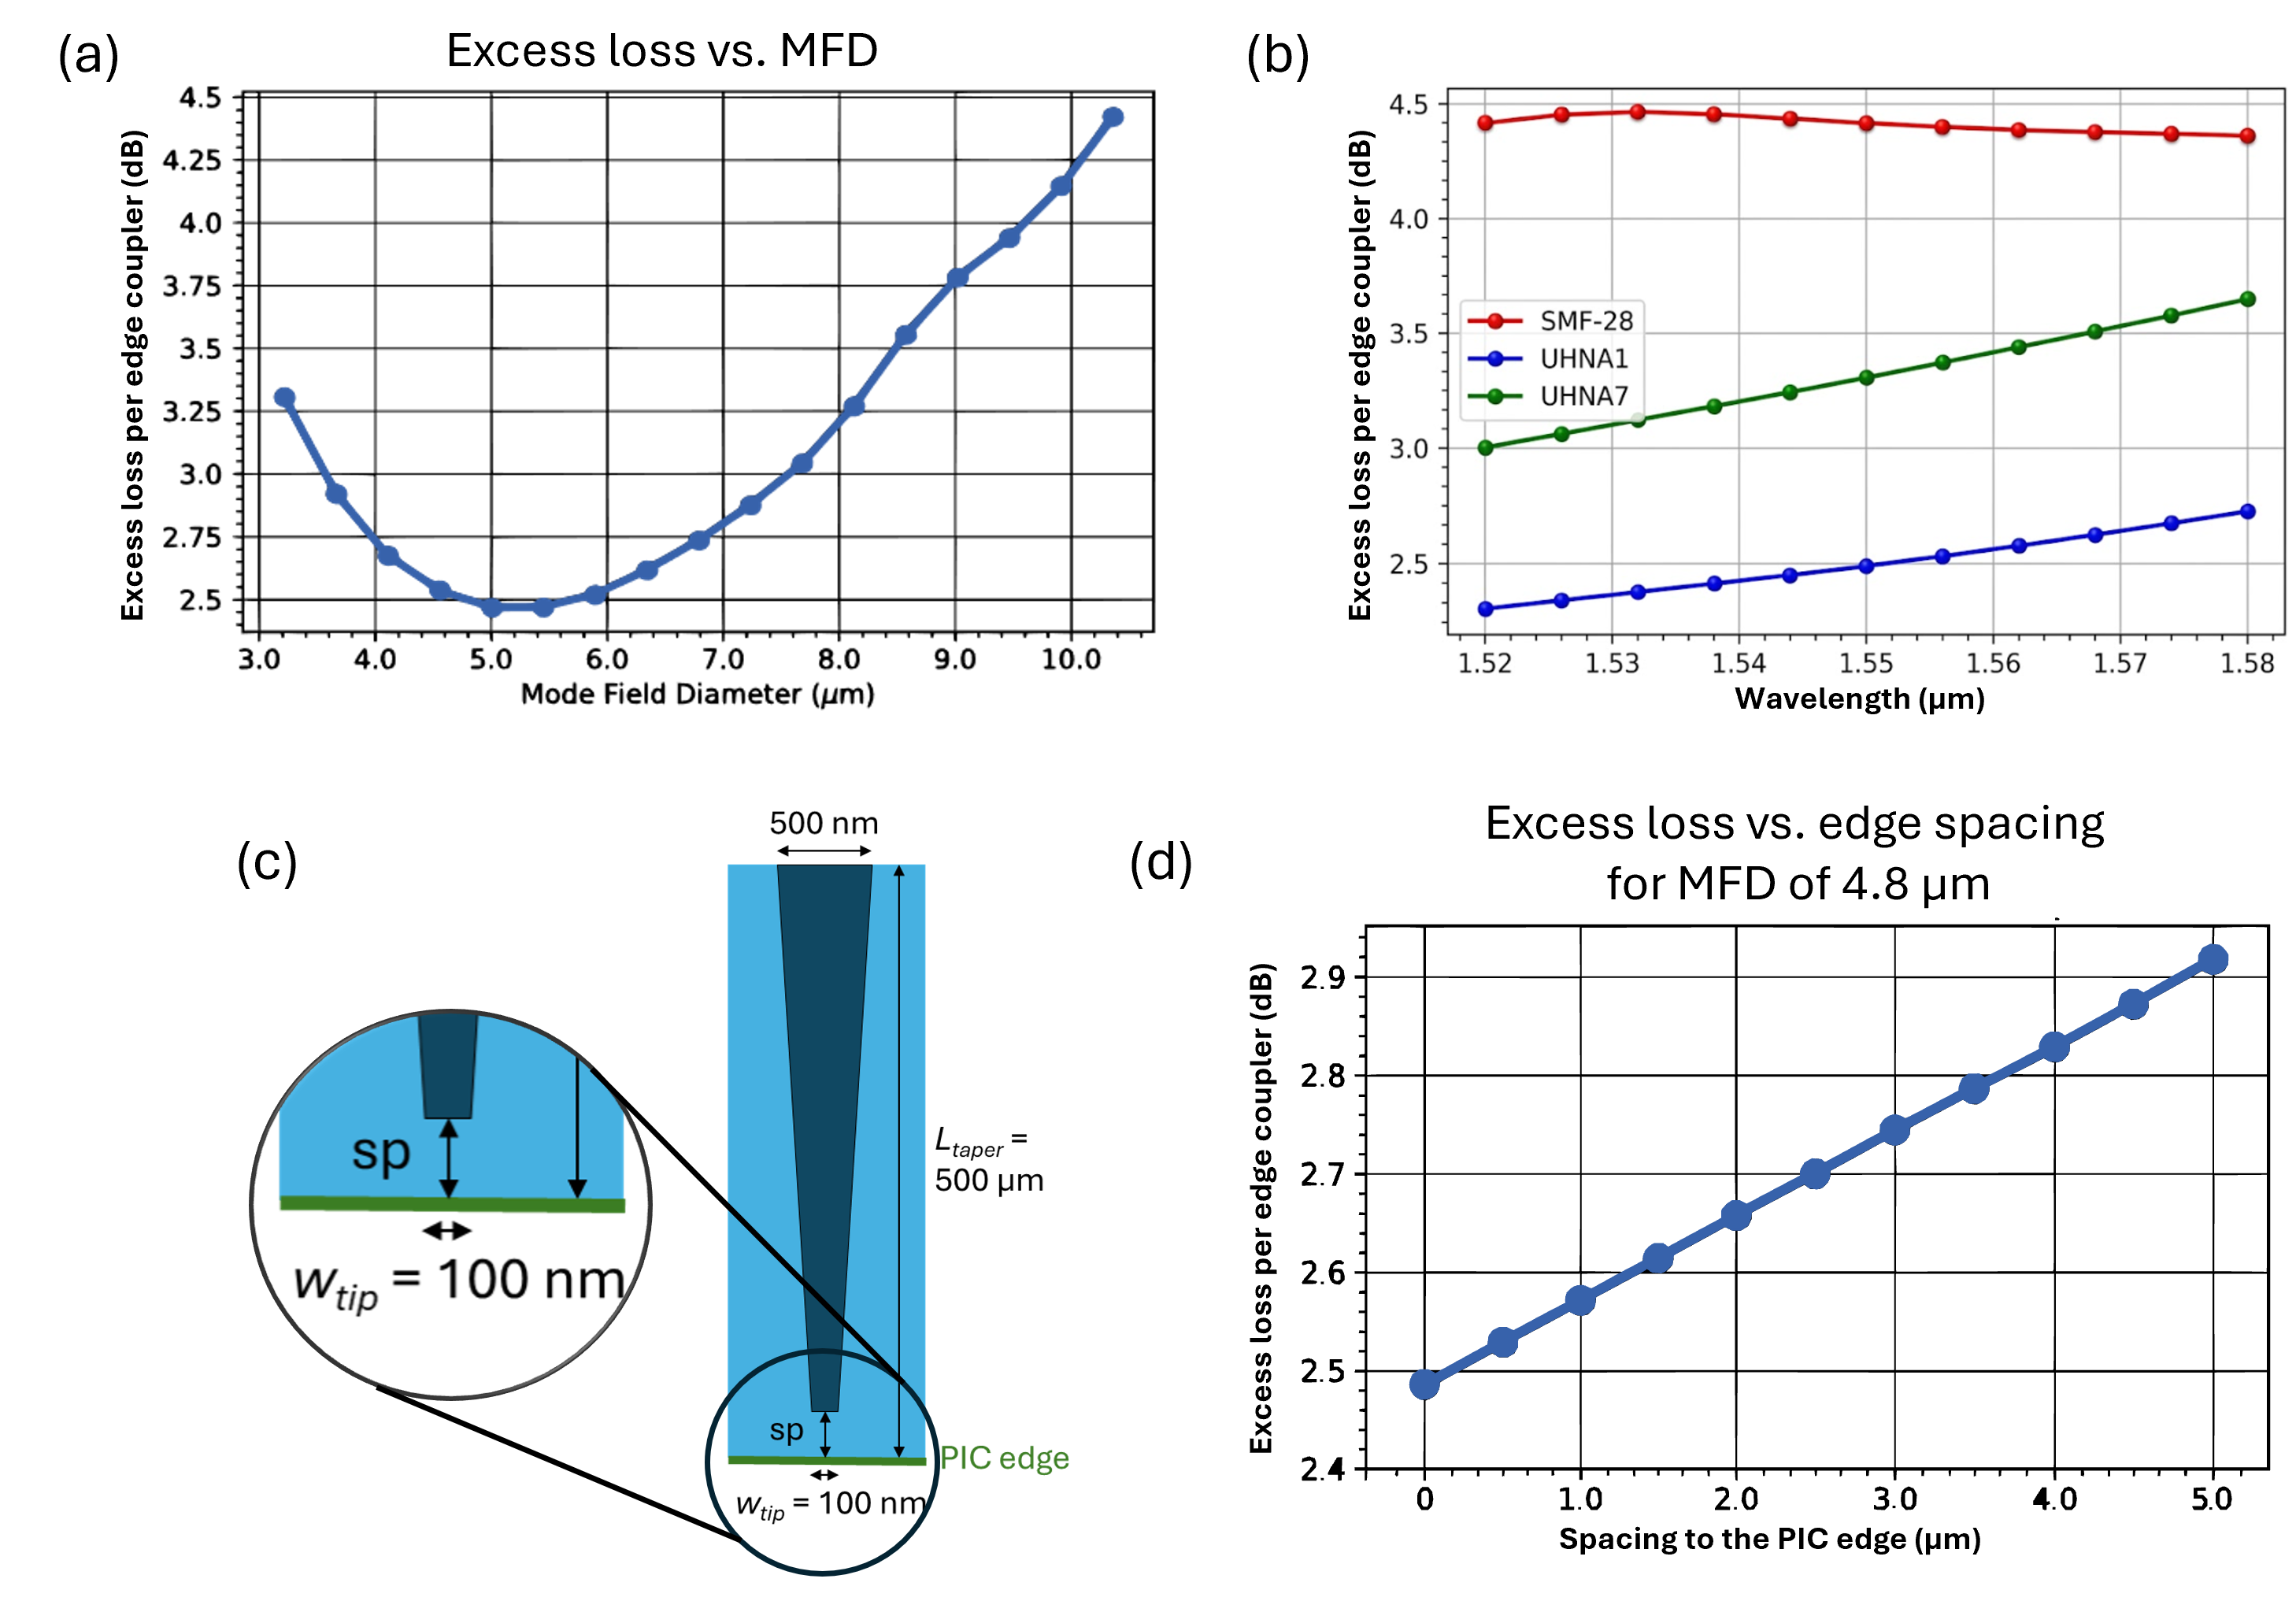
\includegraphics[width=1.0\textwidth]{figures/ch3-edge_coupler_simulations.png}
    \caption{Edge coupler simulation results: (a) Excess loss vs. Mode Field Diameter (MFD). 
    (b) Spectral performance comparison across the C-band for SMF-28, UHNA1, and UHNA7 fibers.
    (c) Schematic representation of the spacing ($sp$) between the PIC facet and the taper tip. 
    (d) Excess loss as a function of $sp$ for a $4.8 \ \mu\text{m}$ MFD.}
    \label{fig:ch3-taper_sims}
\end{figure}

Beyond modal matching, the longitudinal alignment between the taper tip and the chip facet ($sp$) 
was analyzed, as schematized in Figure \ref{fig:ch3-taper_sims}(c). In practice, dicing or 
polishing offsets often prevent the silicon tip from reaching the absolute edge. The simulation for 
the $4.8 \ \mu\text{m}$ MFD case, presented in Figure \ref{fig:ch3-taper_sims}(d), reveals a linear 
increase in loss with a slope of approximately $0.1 \text{ dB}/\mu\text{m}$. This sensitivity 
analysis is critical for the packaging stages described in \nameref{chap:systems}, as it quantifies 
the power budget penalty associated with facet preparation tolerances.

% Despite its modest performance compared to more complex multi-layered or sub-wavelength grating 
% (SWG) tapers, this simple SSC provides the necessary building block for flip-chip compatible 
% architectures. By moving the optical interface to the chip facet, it ensures that the top surface 
% remains available for electrical interconnections and thermal management of active components, 
% fulfilling a critical requirement for the high-density systems characterized in this thesis.



\subsection{Experimental Characterization}

To experimentally validate the performance and dicing tolerances of the proposed designs, a series 
of eight edge coupler (EC) test structures were fabricated. Figure 
\ref{fig:ch3-ec_fabricated}(a) illustrates the layout of these structures, which were arranged in 
a loop-back configuration to facilitate the extraction of the insertion loss per facet.

The set of designs was defined as follows:
\begin{description}
    \item[EC\#3:] Represents the \textbf{nominal design}, corresponding to the optimized parameters 
    derived from the simulation baseline ($sp = 0 \ \mu\text{m}$).
    \item[EC\#1:] Consists of a version \textbf{identical to the nominal design but with a reduced 
    total length}. This variant was included to evaluate the impact of the taper footprint on the 
    coupling efficiency and to verify the adiabaticity of the mode transformation.
    \item[EC\#2, EC\#4, and EC\#5:] Incorporate \textbf{minimal spacing variations}. In these 
    instances, the taper tip was shifted slightly inwards and outwards relative to the theoretical 
    dicing line to evaluate fine fabrication and alignment tolerances.
    \item[EC\#6, EC\#7, and EC\#8:] Involve \textbf{significant offsets}, with the coupler tips 
    retracted approximately $10 \ \mu\text{m}$ from the chip edge. These variations were 
    specifically designed to characterize the impact of more aggressive dicing inaccuracies on the 
    coupling efficiency.
\end{description}

Figure \ref{fig:ch3-ec_fabricated}(b) shows an optical microscope image of the fabricated and 
diced SOI chip. The image confirms the successful definition of the facets and the relative 
positioning of the coupler array within the die. This experimental matrix allows for a direct 
comparison between the theoretical predictions discussed in Section 3.2.1 and the real-world 
performance under typical foundry dicing conditions.

\begin{figure}[!ht]
    \centering
    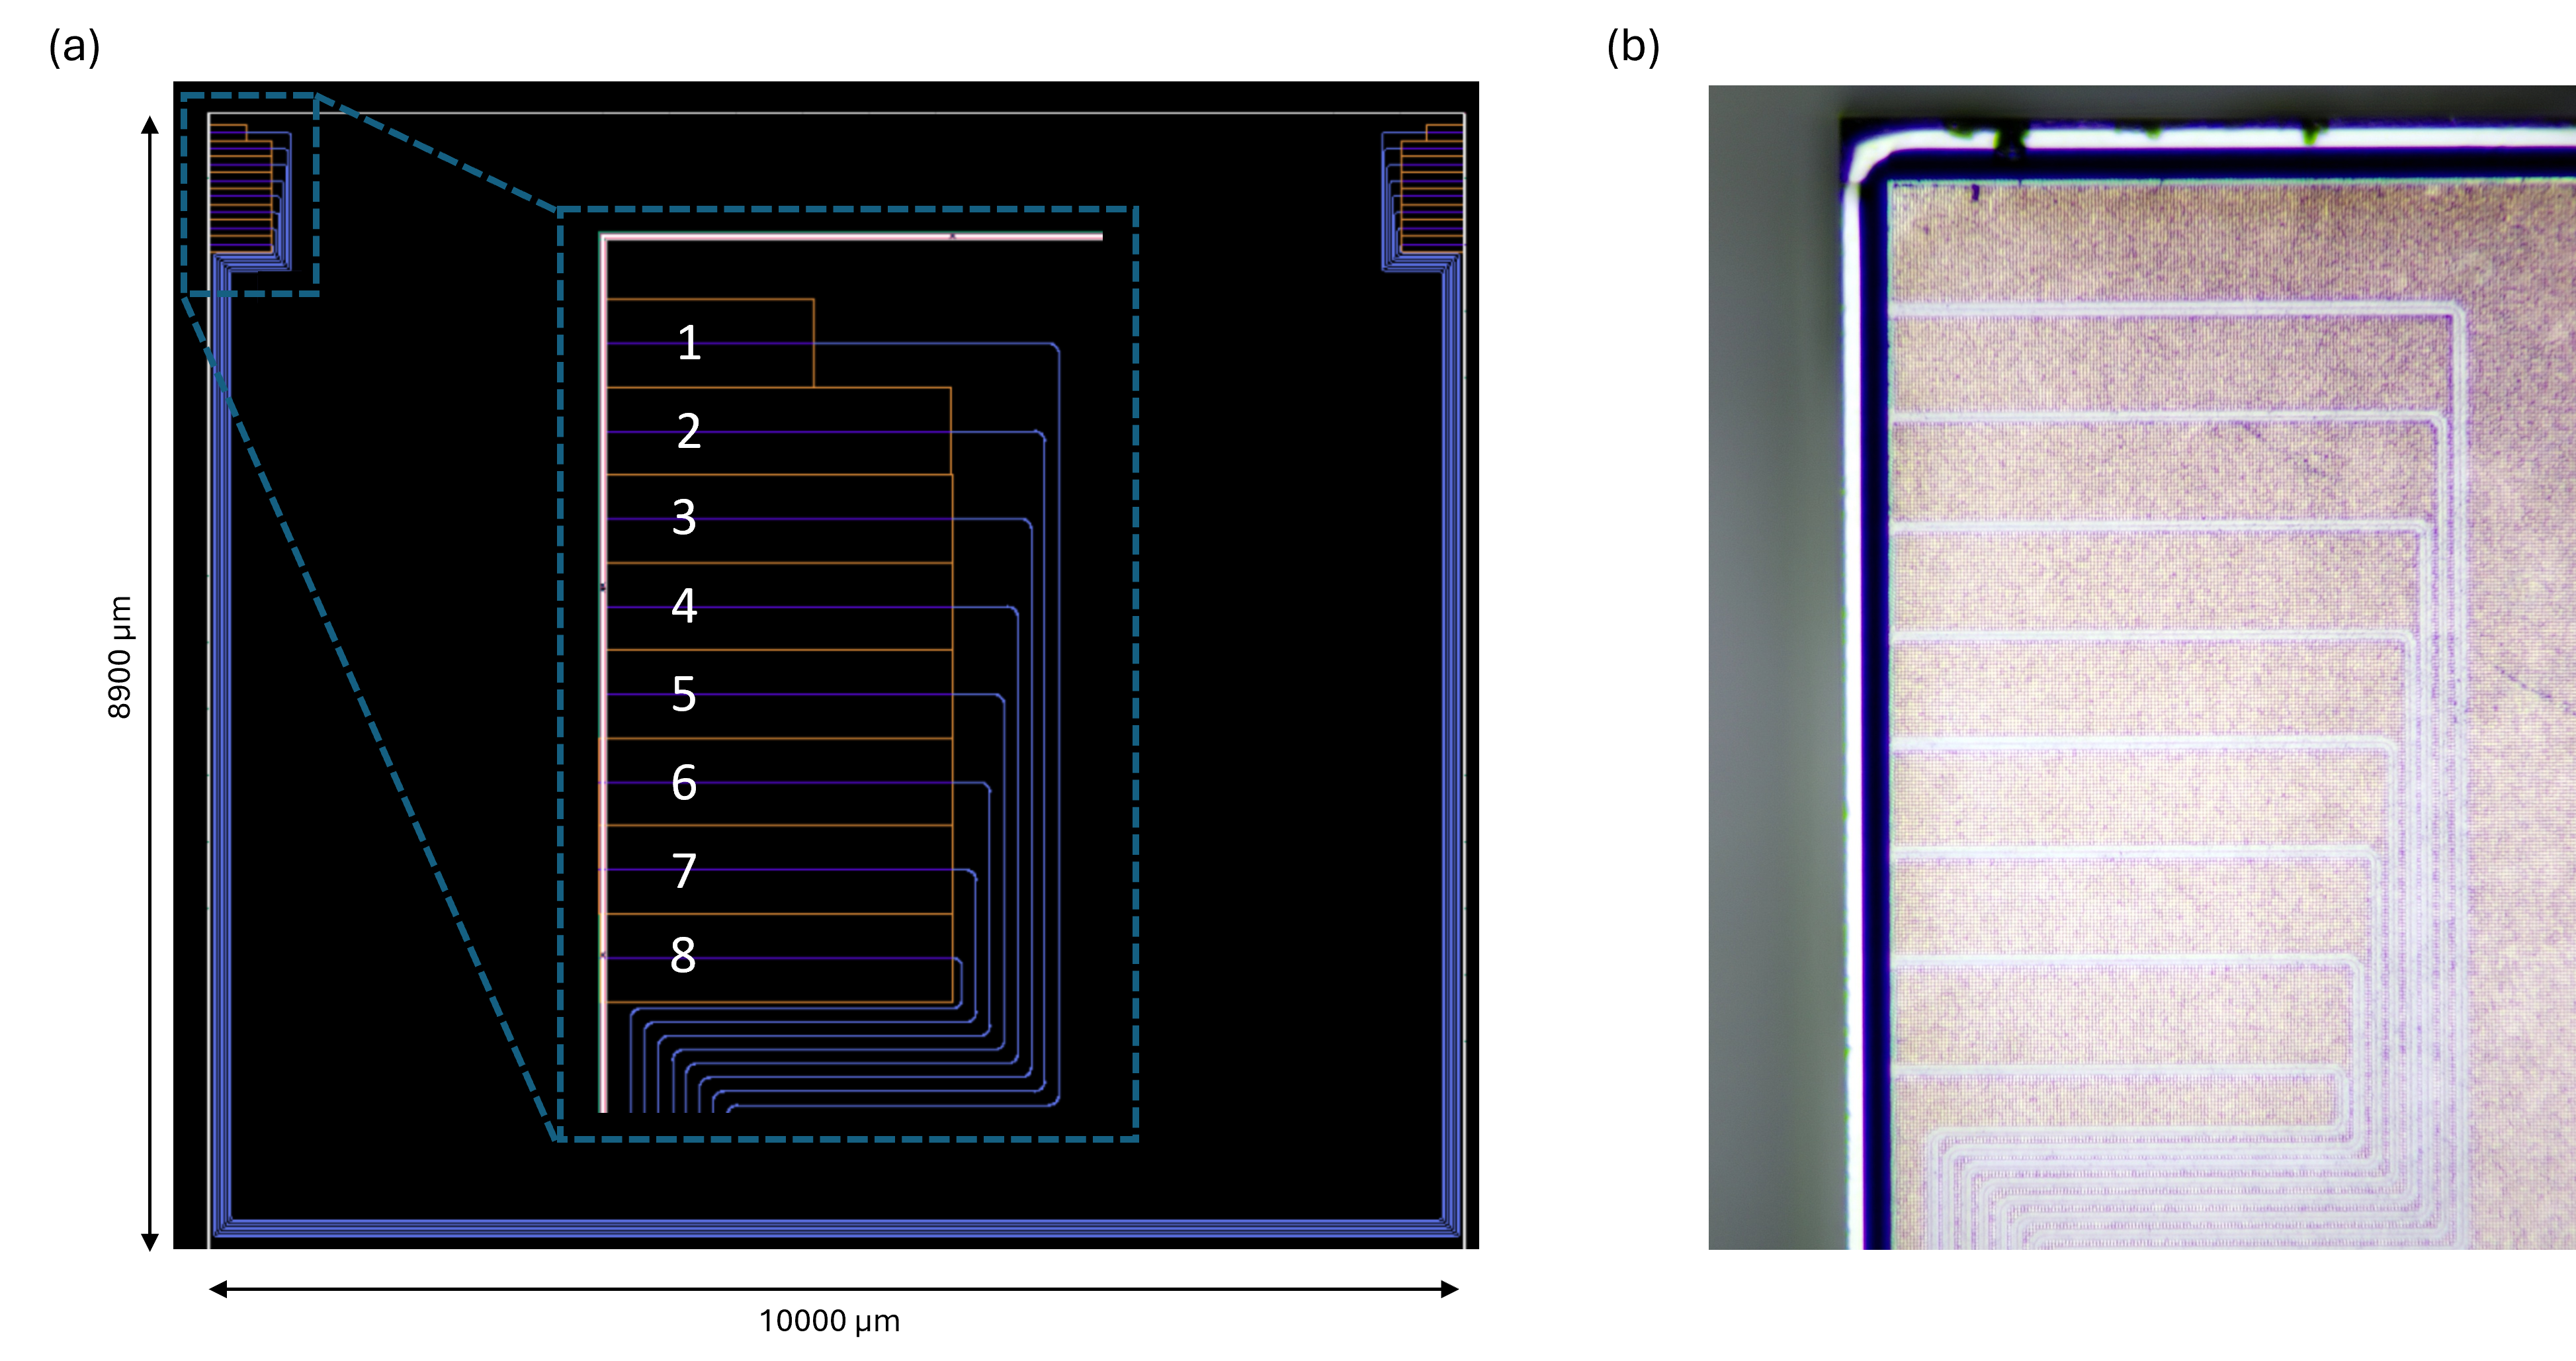
\includegraphics[width=0.8\textwidth]{figures/ch3-edge_coupler_fabricated.png}
    \caption{Experimental validation: (a) Layout of the loop-back test structure and 
    (b) optical micrograph of the fabricated chip facet.}
    \label{fig:ch3-ec_fabricated}
\end{figure}

The spectral response of the fabricated edge couplers was characterized within the $1520-1600 
\text{ nm}$ wavelength range. Figure \ref{fig:ch3-ec_meas} illustrates the experimental results, 
providing a detailed view of the performance and stability of the designs.

Figures \ref{fig:ch3-ec_meas}(a) and \ref{fig:ch3-ec_meas}(b) show the transmission spectra for 
five different DIEs of the nominal design (EC\#3) and the best-performing variant (EC\#7), 
respectively. The high degree of overlap between the curves from different chips demonstrates the 
excellent reproducibility of the fabrication process and the robustness of the inverted taper 
design against chip-to-chip variations.

\clearpage

\begin{figure}[!ht]
    \centering
    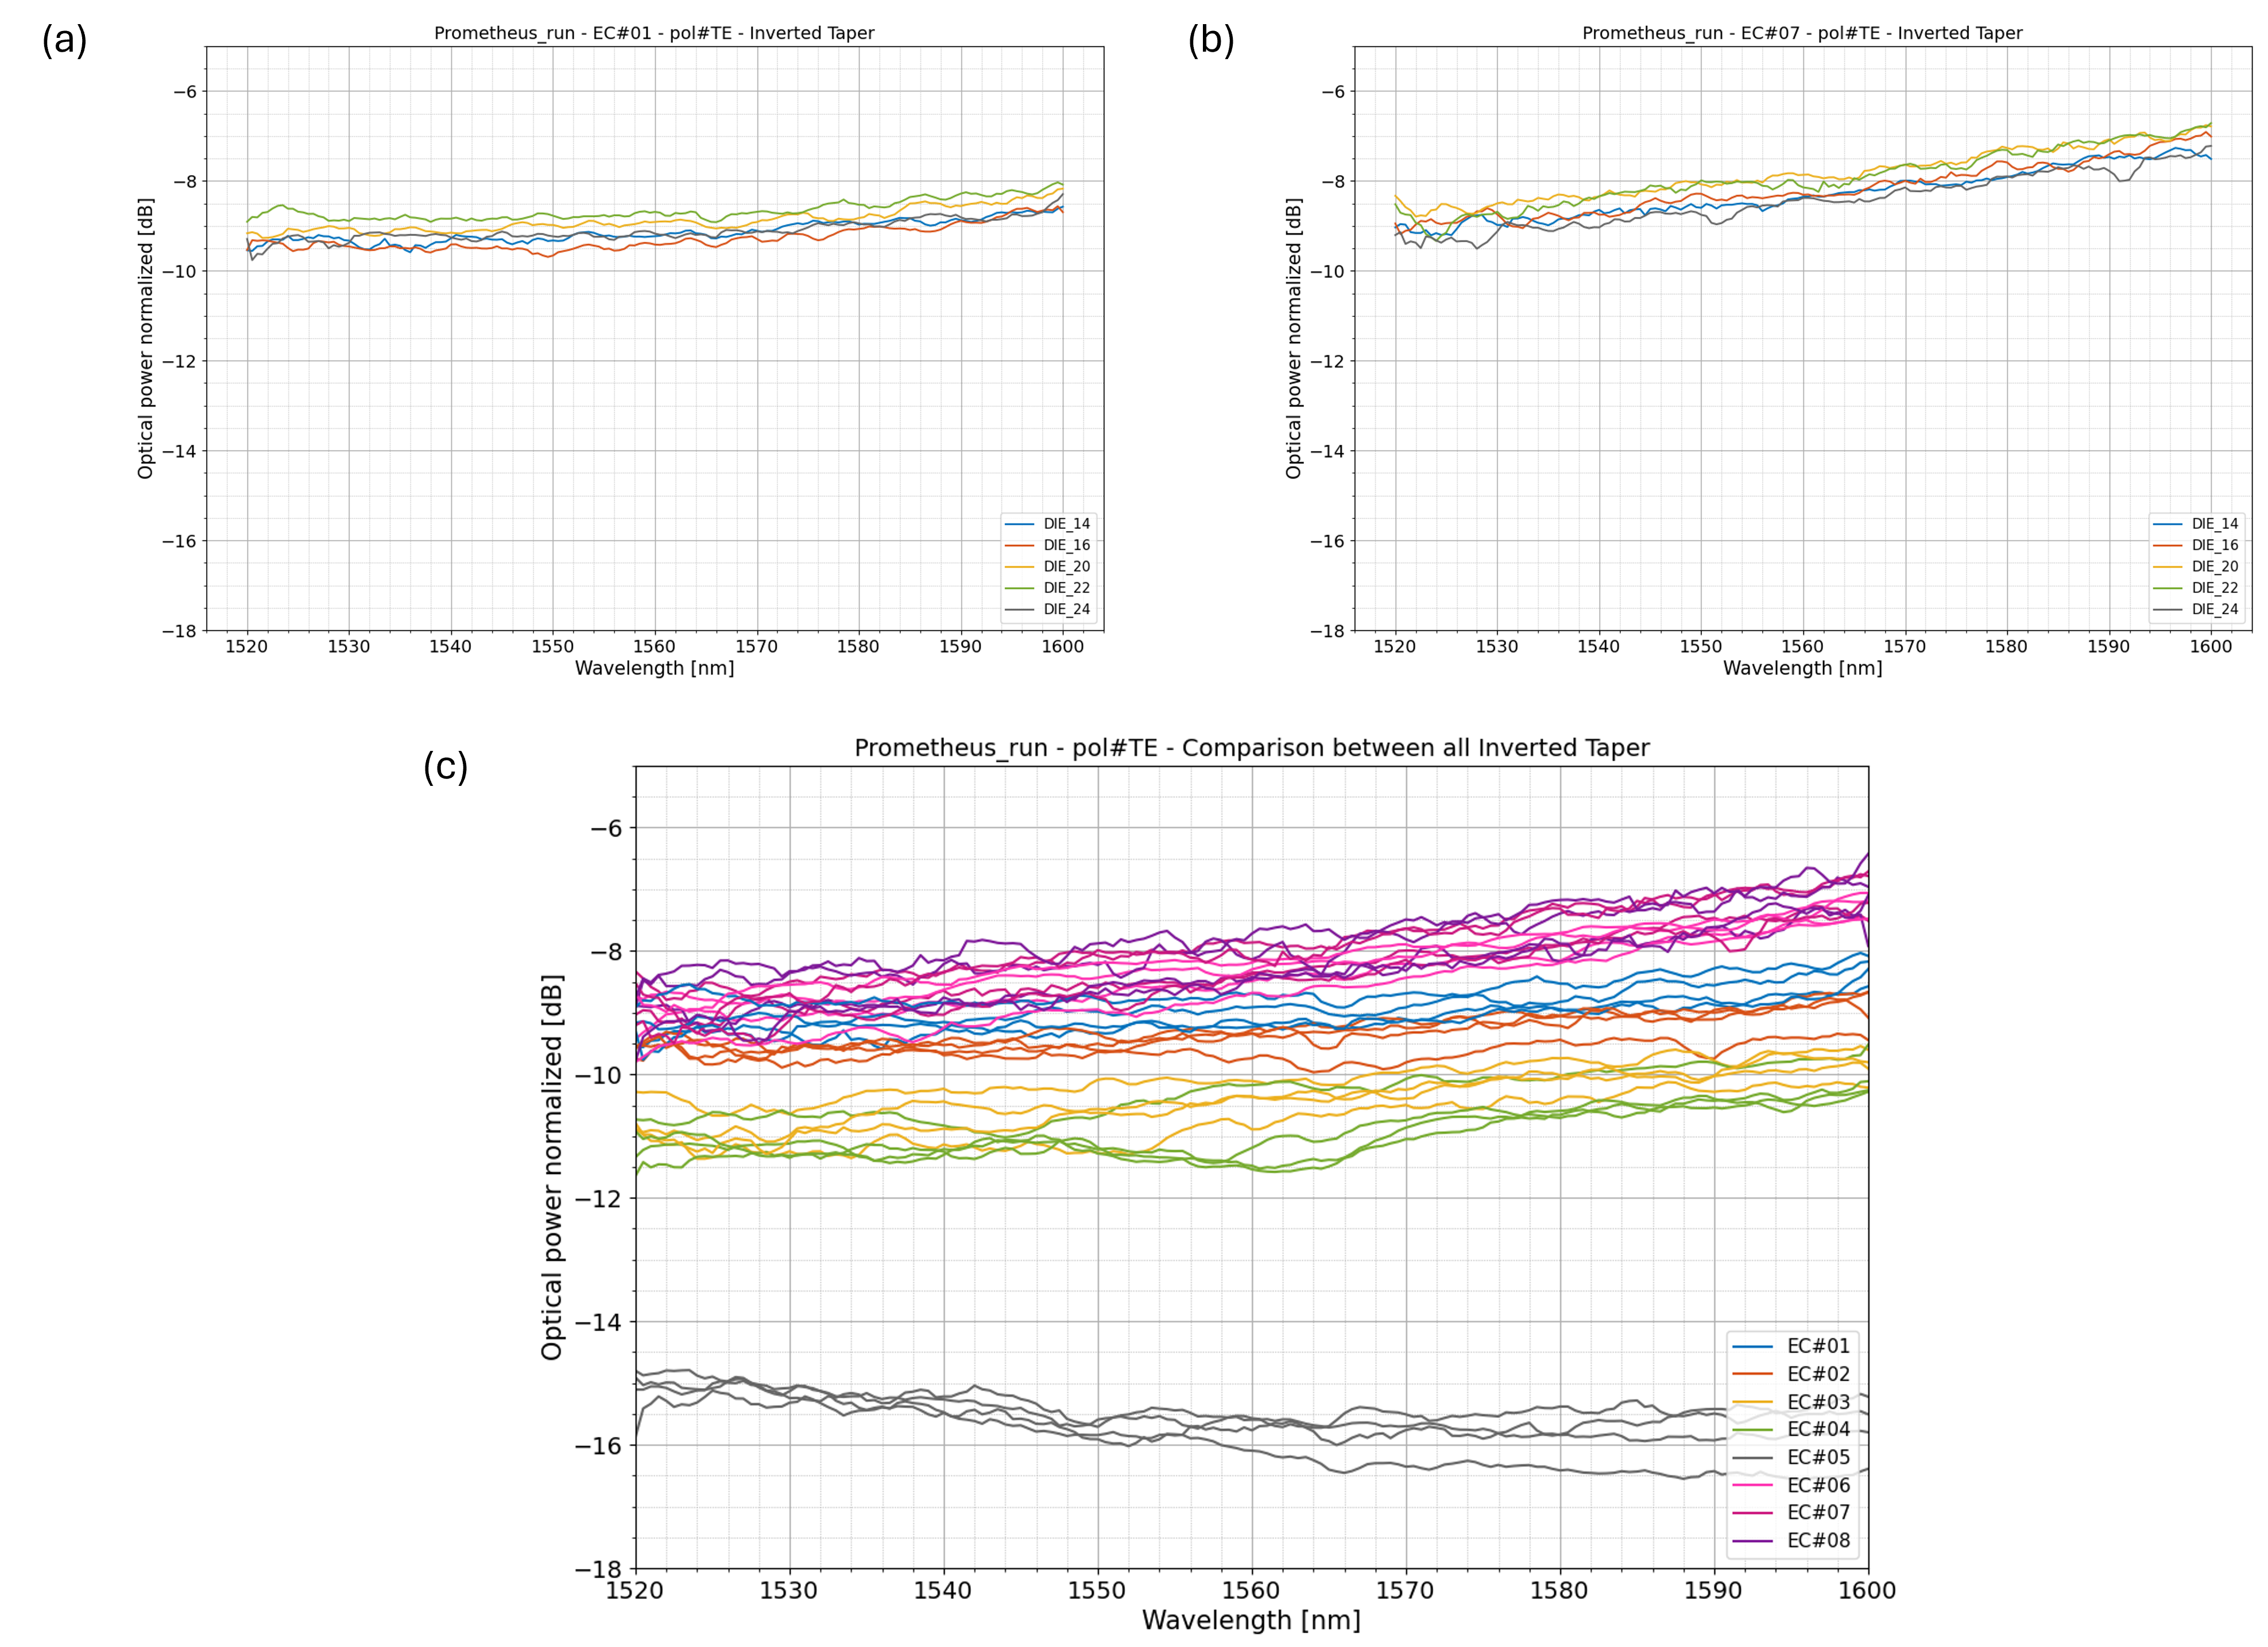
\includegraphics[width=1.0\textwidth]{figures/ch3-edge_coupler_meas_2line.png}
    \caption{Normalized measured optical transmission spectra: (a) EC\#3 and (b) EC\#7 across 5 
    different DIEs showing high reproducibility, and (c) comparison of all eight EC variants.}
    \label{fig:ch3-ec_meas}
\end{figure}


The summarized results, comparing the simulated baseline with the measured performance of these 
devices at $1550 \text{ nm}$, are presented in Table \ref{tab:ec_combined_results}.


\begin{table}[!ht]
\centering
\caption{Comparison between simulated baseline and experimental results at $1550 \text{ nm}$. 
Loss per facet is estimated by dividing the total insertion loss by two.}
\label{tab:ec_combined_results}
\begin{tabular}{lccc}
\toprule
\textbf{Case / Device ID} & \textbf{Total IL (dB)} & \textbf{$\sigma$ (dB)} & \textbf{Loss/Facet (dB)} \\ \midrule
\textit{Simulation (SMF-28)} & 8.80 & --- & 4.40 \\ \midrule
EC\#01 & 9.10  & 0.22 & 4.55 \\
EC\#02 & 9.56  & 0.11 & 4.78 \\
EC\#03 & 10.59 & 0.42 & 5.29 \\
EC\#04 & 11.20 & 0.24 & 5.60 \\
EC\#05 & 15.78 & 0.12 & 7.89 \\
EC\#06 & 8.59  & 0.29 & 4.29 \\
\textbf{EC\#07} & \textbf{8.33} & \textbf{0.33} & \textbf{4.16} \\
\textbf{EC\#08} & \textbf{8.39} & \textbf{0.32} & \textbf{4.19} \\ \bottomrule
\end{tabular}
\end{table}

The experimental results presented in Table \ref{tab:ec_combined_results} lead to several key 
conclusions regarding the edge coupler performance:

\begin{itemize}
    \item \textbf{Validation of the Simulation Model:} The best-performing devices 
    (EC\#7 and EC\#8) achieved insertion losses of approximately $8.33 \text{ dB}$, which is in 
    excellent agreement with the $8.80 \text{ dB}$ predicted by simulations. This slight 
    improvement over the nominal case suggests that the mode expansion and fiber-to-chip alignment 
    were highly optimized during the measurement process.
    \item \textbf{Robustness to Dicing Inaccuracies:} One of the most significant findings is that 
    the designs with a $10 \text{ \mu m}$ retraction (EC\#06--08) showed superior or equivalent 
    performance to the nominal design (EC\#03). This confirms that the inverted taper design is 
    highly resilient to dicing offsets, provided that the mode has enough space to expand before 
    reaching the facet.
    \item \textbf{Adiabaticity and Footprint:} The results for EC\#1 ($9.10 \text{ dB}$) 
    demonstrate that reducing the taper length does not lead to a significant penalty in coupling 
    efficiency. This confirms that the taper profile remains largely adiabatic even in its more 
    compact version, offering a potential path for reducing the total footprint of the PIC.
    \item \textbf{Spectral and Fabrication Stability:} The low standard deviation 
    (under $0.4 \text{ dB}$ for most cases) and the spectral flatness observed across the C-band 
    validate the reliability of the SOI platform and the high-NA fiber interface for broadband 
    applications.
\end{itemize}


% In terms of absolute performance, it must be acknowledged that the measured coupling 
% losses—averaging 4.16--4.55 dB/facet—are relatively high compared to state-of-the-art edge couplers 
% reported in the literature, where values below $1.5 \text{ dB}$ or even sub-decibel performance are 
% common \cite{barwiczAutomatedHighthroughputPhotonic2018, papesFiberchipEdgeCoupler2016, 
% yiPolarizationinsensitiveLowlossOband2025, gaoEfficientSiliconphotonicsEdge2025}.
% This discrepancy is primarily attributed to the lithographic constraints of the dedicated 
% fabrication runs, which limited the minimum taper tip width to $100 \text{ nm}$. As demonstrated in 
% the simulation analysis, this tip width prevents a more effective mode expansion, leading to a 
% significant mode mismatch with the high-NA fiber.

% However, the primary objective of this design was not to achieve record-breaking efficiency, but 
% rather to demonstrate a fault-tolerant interface that enables high-density integration systems, as
% reported in \nameref{chap:systems}. In this regard, the results are highly successful: the coupler 
% maintains a consistent and predictable performance despite significant dicing misalignments of up 
% to $10 \text{ \mu m}$. For applications where assembly reliability and tolerance to mechanical 
% inaccuracies are prioritized over a strict power budget—such as the fault-tolerant PIC architecture 
% proposed in this work—this trade-off between absolute loss and fabrication robustness is justified.

% In conclusion, the edge coupler has been successfully validated as a reliable and resilient entry 
% point for the optical signal. Having established this stable fiber-to-chip interface, the following 
% section describes the design and characterization of the MMI couplers used for on-chip power 
% splitting.

In terms of absolute performance, it must be acknowledged that the measured coupling 
losses—averaging $4.16\text{--}4.55~\text{dB/facet}$—are relatively high compared to 
state-of-the-art edge couplers reported in the literature, where values below $1.5~\text{dB}$ or 
even sub-decibel performance are common \cite{barwiczAutomatedHighthroughputPhotonic2018, 
papesFiberchipEdgeCoupler2016, yiPolarizationinsensitiveLowlossOband2025, 
gaoEfficientSiliconphotonicsEdge2025}. This discrepancy is primarily attributed to the lithographic 
constraints of the dedicated fabrication runs, which limited the minimum taper tip width to 
$100~\text{nm}$. As demonstrated in the simulation analysis, this tip width prevents a more 
effective mode expansion, leading to a significant mode mismatch with the high-NA fiber.

However, the primary objective of this design was not to achieve record-breaking efficiency, but 
rather to demonstrate a fault-tolerant interface that enables high-density integration systems, 
as reported in \nameref{chap:systems}. In this regard, the results are highly successful: 
the coupler maintains a consistent and predictable performance despite significant dicing 
misalignments of up to $10~\mu\text{m}$. For applications where assembly reliability and tolerance 
to mechanical inaccuracies are prioritized over a strict power budget—such as the fault-tolerant 
PIC architecture proposed in this work—this trade-off between absolute loss and fabrication 
robustness is justified.

In conclusion, the edge coupler has been successfully validated as a reliable and resilient entry 
point for the optical signal. Having established this stable fiber-to-chip interface, the following 
section describes the design and characterization of the MMI couplers used for on-chip power 
splitting.


%%%%%%%%%%%%%%%%%%%%%%%%%%%%%%%%%%%%%%%%%%%%%%%%%%%%%%%%%%%%%%
%%%%%%%%%%%%%%%%%%%%%%%%%%%%%%%%%%%%%%%%%%%%%%%%%%%%%%%%%%%%%%


\section{High-Performance MMI via Adjoint Optimization}  

\subsection{Motivation for Inverse Design}
Por qué un MMI estándar no era suficiente (ancho de banda, tamaño o tolerancia)

\subsection{Adjoint Method Implementation}\label{sec:mmi_adjoint}
Explicar brevemente la función objetivo (ej. maximizar transmisión y balance en 1530-1565 nm)

\subsection{Performance Comparison}
Tabla/Gráfica comparando el MMI "analítico" vs. el "optimizado"

\subsection{Experimental Results}
Medidas de Excess Loss e Imbalance





\section{Active Tuning}
Phase Shifter Designs

\subsection{Design of [Thermo-optic/Plasma-dispersion] Shifters}
Geometría del calentador o de la unión PN

\subsection{Static and Dynamic Simulation}
Distribución de calor o perfiles de portadores

\subsection{Experimental Performance}
El valor clave de $P_\pi$ (potencia para desfase de $\pi$), eficiencia y linealidad

\subsection{Chapter Summary (or Concluding Remarks)}
Recapitulación de los mejores resultados obtenidos que se usarán para construir la malla en los siguientes capítulos.

